\problemname{Roomba 1}

\illustration{0.4}{roomba}{Mynd af ryksuguvélmenni eftir \href{https://flic.kr/p/5BrYTp}{geranium alpha}}

Tómas vinur ykkar átti mjög sérvitran afa, herra Miyagi, sem erfði hann af
stórri skemmu á Raufarhöfn. Eina skilyrðið sem afi hans setti var að gólfið í
skemmunni skyldi ávallt vera hreint. Orðrómur hefur lengi verið á kreiki um
hvað sé geymt í skemmunni, en sumir halda að það séu fyrstu 3141 aukastafirnir
í $\pi$. Aðrir halda að skemman geymi Ramsey-töluna $R(6,6)$. Hvað býr þó í
skemmunni verður þó alltaf leyndarmál Tómasar.

Tómas býr í Reykjavík og hefur ekki tíma til að keyra til Raufarhafnar
reglulega til að ryksuga skemmuna. Hann hefur því samband við helstu
ryksugusérfræðinga landsins, en þá er að finna í búðinni \emph{Ryksugur í Úrvali
Með Barka og Allt} (skammstafað RÚMBA) og biður þá um að senda sér öflugasta
ryksuguvélmenni sem þeir hafa yfir að ráða.

RÚMBA fer í að hanna ryksuguvélmenni sem mætir þörfum Tómasar. Eftir þrotlausa
vinnu enda þeir með ryksuguvélmenni sem ryksugar tvöfalt betur og drífur
tvöfalt lengra en nokkuð annað ryksuguvélmenni sem þekkist. Þeir hafa ekki
fundið nafn á það ennþá, en þeir hafa ákveðið að kalla það R2-D2 á meðan þeir
finna betra nafn.

Þeir hjá RÚMBA vilja gera ryksuguvélmennið eins skilvirkt og mögulegt er.
Þ.e.a.s.\ þegar vélmennið ryksugar herbergi, þá vilja þeir hjá RÚMBA ekki að
vélmennið fari óþarflega langa leið.

Hjá RÚMBA vinna engir forritarar og leita þeir því til Tómasar, sem kemur úr
einni frægustu tölvunarfræðingafjölskyldu Íslands, til að útfæra leiðaval
vélmennisins. Tómas er þó of upptekinn við að leysa bakpokaverkefnið í
margliðutíma, svo hann biður ykkur um að útfæra leiðaval vélmennisins fyrir
sig.

Þið fáið þær upplýsingar frá RÚMBA að vélmennið ryksugi bara rétthyrnd herbergi
og að það fær að vita lengd og breidd herbergisins fyrirfram. Vélmennið byrjar
á því að skipta herberginu upp í reiti, þ.e.\ $r$ raðir og $d$ dálka. Vélmennið
velur stærð reitanna á þann hátt að sé það statt í miðjum reit, getur það
ryksugað allan reitinn. Vélmennið gefur hverjum reit hnit $(a,b)$, þar sem $a$
táknar röð reitsins og $b$ dálk hans. Raðirnar eru númeraðar í vaxandi röð frá
botni til topps og dálkarnir frá vinstri til hægri. Byrjað er að telja í núlli.
Sjá dæmi á Mynd~\ref{fig:layout}.

Ykkar verkefni er að finna stystu mögulegu leið fyrir vélmennið að ryksuga allt
herbergið þannig að það endar á sama stað og það byrjar. Vélmennið byrjar
alltaf neðst í vinstra horni herbergisins, þ.e.\ í reitnum $(0,0)$, og getur
aðeins fært sig á milli aðliggjandi reita (en ekki á ská).

\begin{figure}[h!]
    \centering
    % 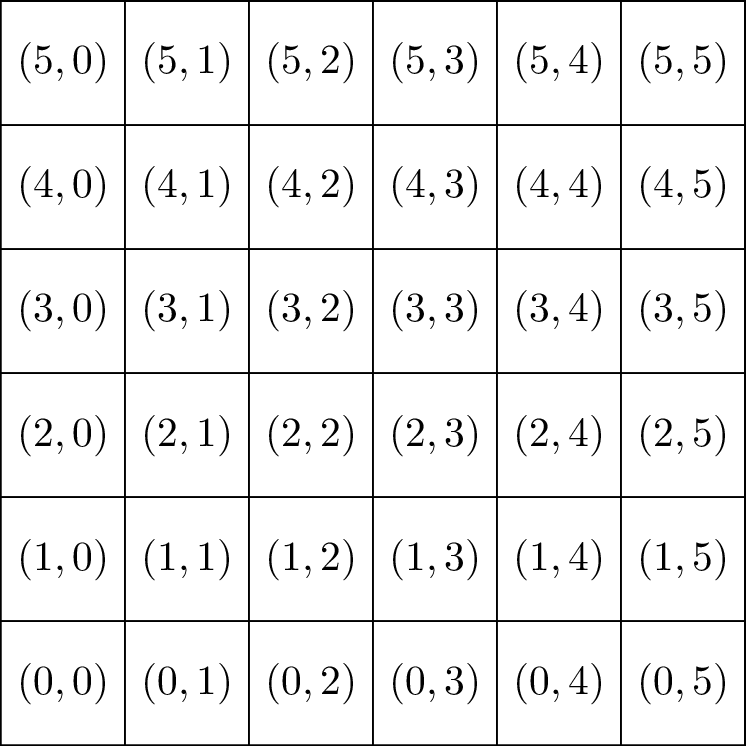
\includegraphics[scale=0.2]{layout.png}
    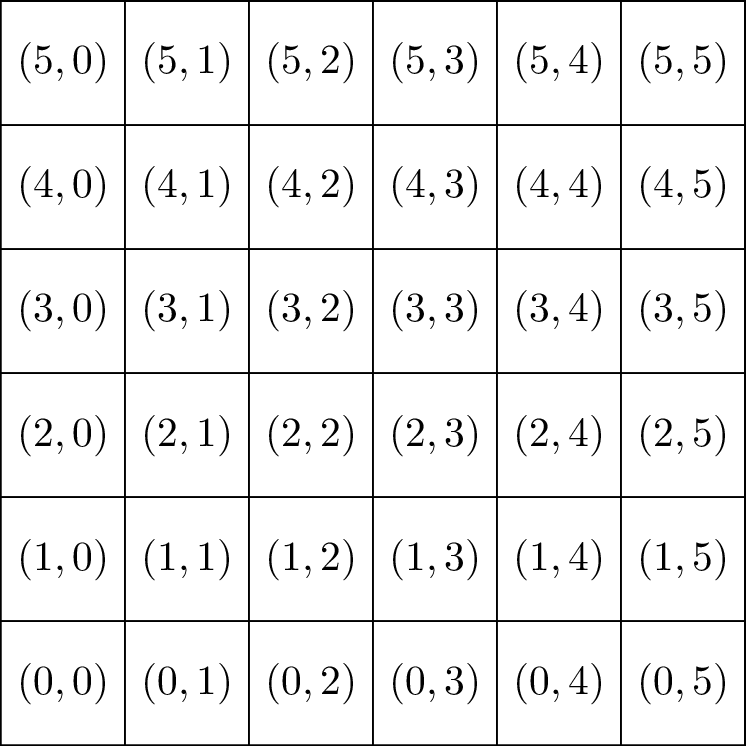
\includegraphics[width=0.7\textwidth]{layout.png}
    \caption{Dæmi um herbergi sem búið er að skipta í $6 \times 6$ reiti.} \label{fig:layout}
\end{figure}


\section*{Inntak}
Inntakið er ein lína sem inniheldur tvær heiltölur, $r$ og $d$, sem táknar að
vélmennið hefur skipt herberginu upp í $r$ raðir og $d$ dálka.


\section*{Úttak}
Skrifið út lengd stystu leiðar sem vélmennið getur tekið til að ryksuga allt
herbergið. Athugið að vélmennið byrjar alltaf á að heimsækja $(0,0)$.


\section*{Stigagjöf}
Lausnin mun verða prófuð á miserfiðum inntaksgögnum, og er gögnunum skipt í
hópa eins og sýnt er í töflunni að neðan. Lausnin mun svo fá stig eftir því
hvaða hópar eru leystir.

\begin{tabular}{| l | l | l | l |}
\hline
Hópur & Stig       & Inntaksstærð          & Önnur skilyrði\\ \hline
1     & 10         & $1 \leq r,d \leq 4$   & \\ \hline
2     & 10         & $1 \leq r,d \leq 5$   & Örlítið þyngri prófunartilvik en í 1 \\ \hline
3     & 20         & $1 \leq r,d \leq 50$  & Örlítið þyngri prófunartilvik en í 1 og 2 \\ \hline
4     & 30         & $1 \leq r,d \leq 100$ & \\ \hline
5     & 30         & $1 \leq r,d \leq 100$ & Örlítið þyngri prófunartilvik en í 4\\ \hline
\end{tabular}
